% $Id$

\chapter{Developing \pyvisi}
\label{chap:developingPyvisi}

In here should be docs on how people can contribute code, modules, renderers
etc to the pyvisi project.

\chapter{Objects and methods defined at base level}

Developers of \pyvisi renderer modules need to provide the classes, subclasses
and methods described below.  They need to be defined with stub classes or
methods even if that functionality is not supported by the rendering backend.
An error or warning message should be given if the user tries to call these
null methods or classes, however they need to be there for completeness.

The most up to date and complete version of this information is contained on
the \pyvisi web site under the documentation page, and then the API link.

\section{Class structure}

The following figure is the class structure of \pyvisi

\begin{figure}
\centerline{%
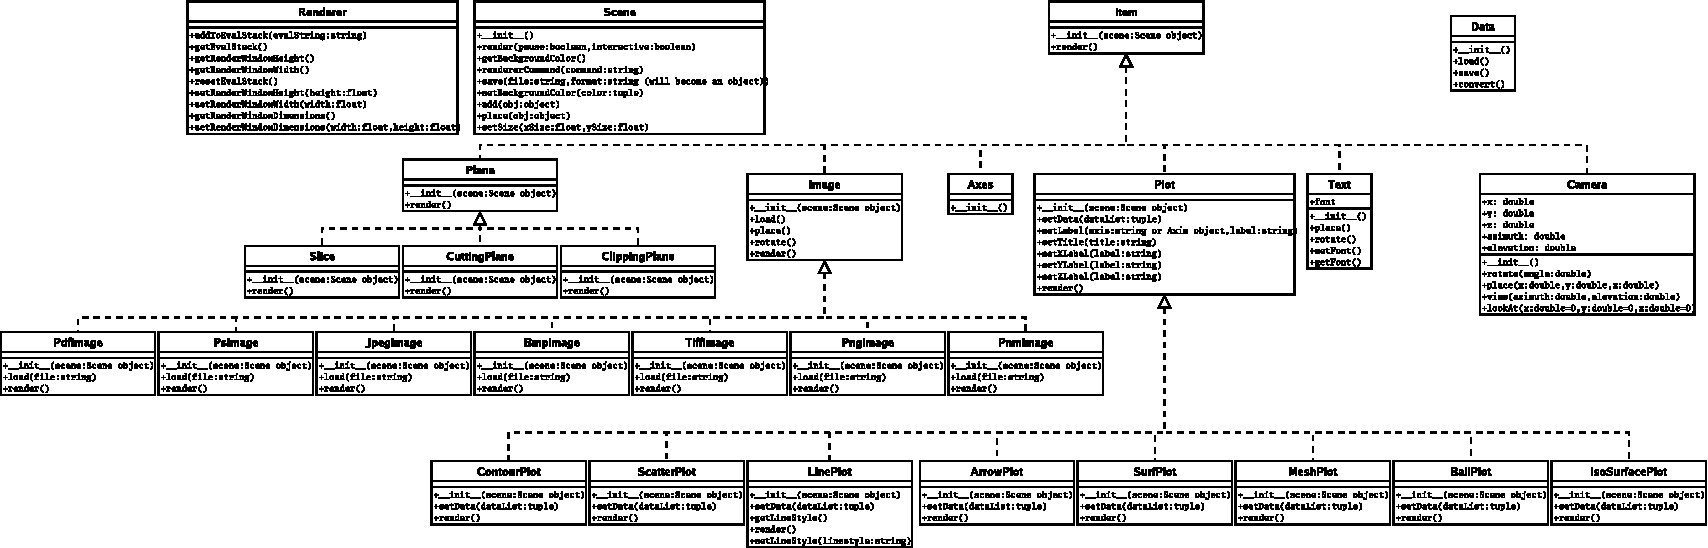
\includegraphics[width=\textheight,angle=90]{figures/pyvisi_class_structure}%
}
\caption{\pyvisi class structure.}
\end{figure}

\section{Fundamental objects}

\subsection{Item}

\subsubsection{render(self)}

Render the object

\subsection{Renderer}

\subsubsection{addToEvalStack(self, evalString)}

Method to add commands to the evaluation stack

\subsubsection{getEvalStack(self)}

Gets the evaluation stack as it currently stands

\subsubsection{getRenderWindowDimensions(self)}

Gets the render window dimensions

\subsubsection{getRenderWindowHeight(self)}

Gets the render window height

\subsubsection{getRenderWindowWidth(self)}

Gets the render window width

\subsubsection{resetEvalStack(self)}

Reset/flush the evaluation stack

\subsubsection{setRenderWindowDimensions(self, width, height)}

Sets the render window dimensions

\subsubsection{setRenderWindowHeight(self, height)}

Sets the render window height

\subsubsection{setRenderWindowWidth(self, width)}

Sets the render window width

\subsection{Scene}

\subsubsection{add(self, obj)}

Add a new item to the scene

\subsubsection{delete(self, obj)}

Delete an item from the scene

\subsubsection{getBackgroundColor(self)}

Gets the current background color setting of the Scene

\subsubsection{getSize(self)}

Gets the current size of the scene

\subsubsection{place(self, obj)}

Place an object within a scene

\subsubsection{render(self, pause, interactive)}

Render (or re-render) the scene

\subsubsection{rendererCommand(self, command)}

Allows the user to run a low-level renderer-specific command directly

\subsubsection{save(self, fname, format)}

Save the scene to a file

\subsubsection{setBackgroundColor(self, *color)}

Sets the background color of the Scene

\subsubsection{setSize(self, xSize, ySize)}

Sets the size of the scene.

\section{Derived objects}

\subsection{Axes}

\subsection{Camera}

\subsection{Image}

\subsubsection{JpegImage}

\subsubsection{PdfImage}

\subsubsection{PngImage}

\subsubsection{PnmImage}

\subsubsection{PsImage}

\subsubsection{TiffImage}

\subsection{Plane}

\subsection{Plot}

\subsubsection{ArrowPlot}

\subsubsection{ContourPlot}

\subsubsection{LinePlot}

\subsection{Text}


%%%%
\chapter{Renderer modules provided by \pyvisi}

\section{vtk}

In the process of being developed.

\section{gnuplot}

In the process of being developed.

\section{povray}

To come.

\section{plplot}

To come.

